\documentclass{report}

\input{~/latex/template/preamble.tex}
\input{~/latex/template/macros.tex}

\title{\Huge{Chapter 2  \\ Exponential and Logarithmic Functions }}
\author{\huge{Matt Warner}}
\date{\huge{}}
\pagestyle{fancy}
\fancyhf{}
\rhead{}
\lhead{\leftmark}
\cfoot{\thepage}
% \usepackage[default]{sourcecodepro} \usepackage[T1]{fontenc}
\usepackage{array}
\usepackage{wasysym}
\pgfpagesdeclarelayout{boxed}
{
  \edef\pgfpageoptionborder{0pt}
}
{
  \pgfpagesphysicalpageoptions
  {%
    logical pages=1,%
  }
  \pgfpageslogicalpageoptions{1}
  {
    border code=\pgfsetlinewidth{1.5pt}\pgfstroke,%
    border shrink=\pgfpageoptionborder,%
    resized width=.95\pgfphysicalwidth,%
    resized height=.95\pgfphysicalheight,%
    center=\pgfpoint{.5\pgfphysicalwidth}{.5\pgfphysicalheight}%
  }%
}

\pgfpagesuselayout{boxed}

\begin{document}
  \maketitle
  \section*{2.1 - Exponential and Logarithmic Functions of the Natural Base, e} 
 \bigbreak \noindent 
 An \textbf{exponential function} is given by

 $$ f(x) = a_0 \cdot a^x$$
 Where 
\bigbreak \noindent
 $$ a > 0 \text{ and } a \neq 1$$
\bigbreak \noindent
 The number a is the base, the y- intercept is $(0, a_0)$, there are no x-intercepts, and the function is continuous for all real numbers.
 \bigbreak \noindent
 While the base of an exponential function may be any positive number except 1, we find that, in calculus, a special number called the \textbf{natural base} is useful.
 \bigbreak \noindent
 To appreciate the usefulness of $e$, consider calculating the future value of an investment that earns compound interest. If P dollars is invested at an annual percentage interest rate $r$ (expressed as a decimal), then the \textit{future value} of the investment after $t$ years, $A(t)$, is given by
 $$ A(t) = P(1 + r )^t$$
 Here, interest is calculated (compounded) once per year. If $n$, called the \textit{compounding frequency}, is the number of times that interest is calculated and added to the amount in an account each year, then the future value is given by
 $$ A = P(1 +\dfrac{r}{n})^{nt}$$
 \bigbreak \noindent
 \hrule
 \bigbreak \noindent
 \q
 \bigbreak \noindent
 \textbf{Luis invests \$5000 in an account that earns interest at an annual rate of 3.25\% Find the future value of Luis's account after 5 yr if interest is compounded (a) annually; (b) quarterly; (c) monthly; and (d) daily.}
  \bigbreak \noindent
  For finding the future value if interest is compounded annually
  \bigbreak \noindent
  We have

  $$ P = \$5000 \ \ \ r = 0.0325 \ \ \ \ t = 5$$
  \bigbreak \noindent
  If interest is compounded annually, we have

  $$ n = 1$$
  \bigbreak \noindent
  So, using the formula

  $$ A = P\left(1 + \dfrac{r}{n}\right)^{nt}$$
  We have, 
  
  $$ A(5) = 5000\left(1 + \dfrac{0.0325}{1}\right)^{ 1(5)}$$

  $$ = \$5867.06$$

  \pagebreak
  \noindent If interest is compounded quarterly (every 3 months), then $n = 4$.
  \bigbreak \noindent
  So,
  
  $$ A(5) = 5000\left(1 + \dfrac{0.0325}{4}\right)^{4(5)}$$
  
  $$ = \$ 5878.38$$
  \bigbreak \noindent
  \bigbreak \noindent
  If interest is compounded monthy, then $n = 12$
  \bigbreak \noindent
  So,
  $$ A(5) = 5000\left(1 + \dfrac{0.0325}{4}\right)^{12(5)}$$

  $$ = \$5880.95$$
  \bigbreak \noindent
  \bigbreak \noindent
  If interest is compounded daily, then $ n = 365$
  \bigbreak \noindent
  So,
  $$ A(5) = 5000\left(1 + \dfrac{0.0325}{4}\right)^{365(5)}$$

  $$ = \$5882.20$$
  \bigbreak \noindent
  \hrule
  \bigbreak \noindent
  From this example, we see that as n increases, the value of Luis's account increases, but not significantly. The increase in value occurs because the interest on the account increases when it is compounded more frequently for the same value of $r$
  \bigbreak \noindent
  Let's consider the expression

  $$ \left(1+\dfrac{1}{n}\right)^n$$
  And explore its value as $n$ increases. 
  \bigbreak \noindent
    \renewcommand{\arraystretch}{1.5}
    \begin{table}[h]
    \begin{center}
        \begin{tabular}{|c|c|}
            \hline
            $n$ & $\left(1+\frac{1}{n}\right)^n$ \\
            \hline
            10 & $\left(1+\frac{1}{10}\right)^{10}=2.59374246 \ldots$ \\
            100 & $\left(1+\frac{1}{100}\right)^{100}=2.704813829 \ldots$ \\
            1000 & $\left(1+\frac{1}{1000}\right)^{1000}=2.716923932 \ldots$ \\
            10,000 & $\left(1+\frac{1}{10,000}\right)^{10,000}=2.718145926 \ldots$ \\
            100,000 & $\left(1+\frac{1}{100,000}\right)^{100,000}=2.718268237 \ldots$ \\
            \hline
        \end{tabular} 
  \end{center} 
    \end{table}
\bigbreak \noindent
As $n$ approaches $\infty$, growth continuously, and $\left(1 + \dfrac{1}{n}\right)^n$ gets closer to a number approximated by 2.718.... We call this number the \textit{natural base}, denoted $e$.

\pagebreak
\noindent
Now consider

$$ P \left(1+\dfrac{r}{n}\right)^{nt}$$
And let $m = \dfrac{n}{r}$ so that $ n = mr$. Substituting, we have
$$ P \left(1+\dfrac{r}{n}\right)^{nt} = P \left(1 + \dfrac{r}{mr}\right)^{mrt} = P \left(1 + \dfrac{1}{m}\right)^{mrt}$$
\bigbreak \noindent
As $n \to\infty$, then $m \to\infty$ also. Thus,

$$ \displaystyle\lim_{n\to\infty}\left[P\left(1+\dfrac{r}{n})^{nt}\right] = \displaystyle\lim_{m\to\infty}\left[P\left(1+\dfrac{1}{m}\right)^{mrt}\right]$$
\bigbreak \noindent
\noindent At this point, the variable $m$ is no longer needed, and we have the following result.
\bigbreak \noindent
\thm{}{
  A quantity P, growing continuously at annual percentage rate $r$, expressed as a decimal, has a future value after $t$ years given by
  $$ Pe^{rt}$$
}
\q
\bigbreak \noindent
\textbf{Luis invests \$5000 in an account that earns interest at an annual rate of 3.25\%. Find the future value of Luis's account after 5 yr if interest is compounded continuously.}
\bigbreak \noindent
We have,

$$ P = \$5000 \ \ \ r = 0.0325 \ \ \ t = 5$$
So,

$$A = 5000e^{0.0325{5}}$$
$$ = \$ 5882.24$$
\bigbreak \noindent
The graphs of $f(x) = e^x$ and $g(x) = e^{-x}$ are shown below. Both functions have the domain $(-\infty, infty)$, the range $(0,\infty)$, the y-intercept $(0,1)$, and no x-intercepts. As x increases in value, $e^x$ increases in value without bound, but $e^{-x}$ decreases toward 0 as a limit. That is
% $$ \displaystyle\lim_{x\to\infty}e^{-x} = 0$$
\bigbreak
\hspace{-4mm}\begin{minipage}{0.46\textwidth}
    \centering
    \incfig[1]{ex}
  \end{minipage}
  \begin{minipage}{0.5\textwidth}
    \incfig[1]{naa}
  \end{minipage}
  \begin{mdframed}
\subsection*{The Natural Logarithm}
\bigbreak \noindent
Recall that 

$$ \log_{a}x = y$$
Can be rewritten as

$$ a^{y} = x$$
\bigbreak \noindent \bigbreak \noindent
We now introduce the logarithm, base e, called the \textbf{natural logarithm} and denoted $\mathbf{\ln}$
\bigbreak \noindent
\subsection*{Definition}
For any positive number x, the \textbf{natural logaritm} or \textbf{logarithm, base e,} of x, is given b

$$ \ln x = \log_{e}x$$
The equation $ y=\ln x$ is equivalent to 

$$e^y = x$$
\vspace{0.5mm}
\end{mdframed}
\bigbreak \noindent
\q
\bigbreak \noindent
\textbf{Find each of the following. If necessary, use a calculator to approximate values to three decimal places.}
\bigbreak \noindent
\textbf{Problem 1.} Find $\ln e^3$
\bigbreak \noindent
\textbf{\textit{Since}}

$$ y = \ln{x} \ \ = \ \ e^y = x$$
\textit{\textbf{Then}}

$$ \ln{3} = \ \ e^y = e^3$$
\textit{\textbf{So}}

$$ 3 = y$$
\bigbreak \noindent
\textbf{Problem 2.} Find ln 1
\bigbreak \noindent
\textit{\textbf{Since}}

$$ \ln{1} \ \ = \ \ e^y = 1$$
\bigbreak \noindent
\textit{\textbf{We need to find the power of e that gives 1.}}
\bigbreak \noindent
\textit{\textbf{Thus}}
$$y = \ln{1} = 0$$
\pagebreak 
\thm{}{
  Properties of Natural Logarithms
  \bigbreak \noindent
  \textit{\textbf{P1.}} $\ln{MN} = \ln{M} + \ln{N}$ \hspace{16.5mm} \textit{\textbf{P5.}} $\ln{1} = 0$
  \bigbreak \noindent
\textit{\textbf{P2.}} $\ln{\dfrac{M}{N}} = \ln{M} - \ln{N}$ \hspace{18mm} \textit{\textbf{P6.}} $\log_bM = \dfrac{\ln{M}}{\ln{b}}$ 
  \bigbreak \noindent
  \textit{\textbf{P3.}} $\ln{M^k} = k \cdot \ln{M}$ \hspace{23mm} \textit{\textbf{P7.}} $\ln{e^x} = x, \text{ for all real numbers x}$
  \bigbreak \noindent
  \textit{\textbf{P3.}} $\ln{e} = 1$ \hspace{37mm} \textit{\textbf{P8.}} $e^{ln{x}} = x$, for all $x > 0$
}
\bigbreak \noindent
\q
\bigbreak \noindent
\textbf{Given} 
$$\mathbf{ln{\ 2} = 0.6931 \ \ \ \ and  \ \ \ \ ln{\ 3} = 1.0986}$$
\vspace{1mm}

\noindent\textbf{Use the properties of natural logarithms to find each of the following}
\bigbreak \noindent
\textbf{Problem 1.} Find $\ln{6}$
\bigbreak \noindent \bigbreak \noindent
\textit{\textbf{We can rewrite this as}}

$$\ln{(2 \cdot 3)}$$
\textit{\textbf{This equates to}}

$$ \ln{2} + \ln{3}$$
\textit{\textbf{which is}}

$$ 0.6931 + 1.0986$$
$$ = 1.7917$$
\bigbreak \noindent
\textbf{Problem 2.} Find $\ln{81}$
\bigbreak \noindent \bigbreak \noindent
\textit{\textbf{We can rewrite this as}}

$$\ln{3^4}$$
$$ = 4\ln{3}$$
\textit{\textbf{This equates to}}

$$ 4(1.0986)$$
$$ = 4.3944$$
\bigbreak \noindent
\textbf{Problem 3.} Find $\ln{\dfrac{1}{3}}$
\bigbreak \noindent
\textit{\textbf{Using property P1.}}
$$ \ln{\dfrac{1}{3}} = \ln{1} - \ln{3}$$
$$ = 0 - 1.0986$$
$$ = -1.0986$$

\pagebreak
\noindent There are two ways in which we might graph 
$$y = f(x) = \ln{x}$$
One is to graph the equivalent equation 
$$x = e^y$$ 
by selecting values for y and calculating the corresponding values of $e^y$. We then plot points, remembering that x is still the first coordinate.
\bigbreak noindent
\begin{minipage}{0.5\textwidth}
    \incfig[1]{workdammit}
\end{minipage}
\begin{minipage}{0.5\textwidth}
    \incfig[1]{tyyyyy}
\end{minipage}
\begin{figure}[ht]
    \centering
    %\caption{workdammit}
    %\label{fig:workdammit}
\end{figure}
\begin{figure}[ht]
    \centering
    %\caption{tyyyyy}
    %\label{fig:tyyyyy}
\end{figure}
\bigbreak \noindent
The graph above shows that graph of $g(x) = e^x$ for comparison with that of $f(x) = \ln{x}$.
\bigbreak \noindent
\nt{
  Note that the functions are inverses of each other. That is, the graph of $y=\ln{x}$, or $x = e^y$, is a reflection across line $ y=x$ of the graph of $y=e^x$
  \bigbreak \noindent
  Any ordered pair (a,b) on the graph of g yeilds an ordered pair (b,a) on $f$
  \bigbreak \noindent
  A second method of graphing $y=\ln{x}$ is to use a calculator to find function values. For example, when x = 2, then  $y = \ln{2} \approx 0.6931$. This gives the pair (2,0.6931) shown on the graph.
}
\bigbreak \noindent
The following properties can be observed from the graph.
\bigbreak \noindent
\thm{}{
  $\ln{x}$ exists only for positive numbers x. The domain is $ (0,\infty)$
  \bigbreak \noindent 
  $$\ln{x < 0}, \text{ for } 0 < x < 1;$$
  $$ \ln{x = 0}, \text{ for } x = 1;$$
  $$ \ln{ x > 0}, \text{ for } x > 1.$$
\bigbreak \noindent
The function given by $f(x) = \ln{x}$ is always increasing. The range is the entire real line, $(-\infty,\infty)$, or the set of real numbers, $\mathbb{R}$
}
\pagebreak
\nt{
  Note that for an expression such as $\ln{(x-2)}$, we require that $x - 2 > 0$ or, equivanlently, $ x > 2$
  \bigbreak \noindent
  Thus, the domain of $ y=\ln{(x-2)}$ is $(2,\infty)$
}
\bigbreak \noindent
\q
\bigbreak \noindent
\textbf{Find the domain of \mathbf{f(x) = ln(5-2x)}}
\bigbreak \noindent
\textit{\textbf{We require that 5 - 2x be positive. That is, we must have}}
$$ 5 - 2x > 0$$

$$-2x>-5$$

$$x<\dfrac{5}{2}$$
\vspace{1mm}

\noindent \textbf{\textit{Thus, the domain of $f$ is}}

$$ \left(-\infty, \dfrac{5}{2}\right)$$
\bigbreak \noindent \bigbreak \noindent
\hrule
\bigbreak \noindent
\section*{Solving Exponential and Logarithmic Equations, Base e}
A common method for solving exponential equations is to find the natural logarithm of both sides. We first isolate the exponential term, then write the equivalent logarithmic forms of the equation.
\bigbreak \noindent
$$ e^x = b$$
$$ \ln{e^x = \ln{b}}$$
$$ x = \ln{b}$$
\bigbreak \noindent
\q
\bigbreak \noindent
\textbf{Solve:} $\mathbf{e^{3x} = 2}$
\bigbreak \noindent 
\vspace{2mm}

\noindent\textit{\textbf{Take the natural log of both sides}}

$$ \ln{e^{3x}} = \ln{2}$$

$$ 3x = \ln{2}$$

$$ x = \dfrac{\ln{2}}{3}$$

$$ \approx 0.231$$

\pagebreak
\q
\bigbreak \noindent
\textbf{Marisa invests \$12,000 in an account that earns 2.8\% annual interest, compounded continuously. When will Marisa's account double in value.}
\bigbreak \noindent
\textit{\textbf{The value of Marisa's account after $\mathbf{t}$ years is given by}}

$$ A(t) = 12,000e^{0.028t}$$
\textit{\textbf{So to find find when it doubles,}}

$$24,000 = 12000e^{0.028t}$$
\textit{\textbf{divide both sides by 12000}}

$$ 2 = e^{0.028t}$$
\textit{\textbf{Take the natural log of both sides}}

$$ \ln{2} = \ln{e^{0.028t}}$$
$$  \ln{2} = e^{0.028t}$$
$$ t = \dfrac{\ln{2}}{0.028} \approx 24.8 \ yr.$$
\bigbreak \noindent
This suggests a general formula for finding the time needed for an inital quantity $P$ to double in size.
\bigbreak \noindent
Letting T represent the doubling time, we have
$$ 2P = Pe^{rT}$$
$$ 2 = e^{rT}$$
$$\ln{2} = \ln{e^{rT}}$$
$$ \ln{2} = {rT}$$
\bigbreak \noindent
\nt{
  Note that since this relationship between $r$ and $T$ does not depend on $P$. It takes as long for \$1 to double as it does for \$10,000 to double.
}
\bigbreak \noindent
\thm{}{
  The \textbf{exponential growth rate r} (expressed as a decimal) and the \textbf{doubling time} T are related by
  $$ rT = \ln{2}, \ \ \ \ \ or \ \ \ \ \ r = \dfrac{\ln{2}}{T} \ \ \ \ and \ \ \ \ T = \dfrac{\ln{2}}{r}$$
}
\pagebreak
\section*{Derivatives of Exponential Functions}
To find the derivative of the exponential function
$$ f(x) = e^x$$
We use the definition of the derivative given by
$$ f'(x) = \displaystyle\lim_{h\to 0}\dfrac{f(x+h)-f(x)}{h}$$
$$ = \displaystyle\lim_{h\to 0}\dfrac{e^{x+h} - e^x}{h}$$
$$ = \displaystyle\lim_{h\to 0}\dfrac{e^x \cdot e^h - e^x \cdot 1}{h}$$
$$ = \displaystyle\lim_{h\to 0} \left(e^x \cdot \dfrac{e^h - 1}{h}\right)$$
$$ = e^x \cdot \displaystyle\lim_{h\to 0}\dfrac{e^h-1}{h}$$
\textit{\textbf{Thus}}
$$f'(x) = e^x \cdot \displaystyle\lim_{h\to 0}\dfrac{e^h -1}{h}$$
\bigbreak \noindent
Using a calculator, we find that
$$ \displaystyle\lim_{h\to 0}\dfrac{e^h -1}{h} - 1$$
\textit{\textbf{Thus,}}
$$f(x) = e^x$$
Then its derivative is
$$ f'(x) = e^x$$
\bigbreak \noindent
This remarkable result is summarized in the following theorem.
\bigbreak \noindent
\thm{}{
  The derivative of the function $f$ given by
  $$ f(x) = e^x$$
  is the function itself.
  $$ f'(x) = f(x), \ \ \ \ or \ \ \ \ \frac{d}{dx}e^x = e^x$$
}
  \bigbreak \noindent
  \begin{minipage}{0.5\textwidth}
  Theorem 0.5 says that for	
  $$f(x) = e^x$$
  The derivative at x (the slope of the tangent line) \\ is the same as the function value at x.
  \bigbreak \noindent
  That is, on the graph of
  $$f(x) =e^x$$
  For reference,
  \\ 
  At the point (0,1), the slope is m = 1; \\
  \vspace{0.5mm}

  At the point (1,e), the slope is $m = e$
  \end{minipage}
  \begin{minipage}{0.5\textwidth}
    \vspace{10mm}\incfig[1]{hghghg}
  \end{minipage}
  \pagebreak
  \section*{Finding Derivatives of Functions Involving e}
  We can combine Theorem 5 with earlier theorems to differentiate a variety of functions.
  \bigbreak \noindent
  \q   $$\text{\textbf{Find}} \ \  \mathbf{\frac{dy}{dx}}$$
  \bigbreak \noindent
  \textbf{Problem 1.} $ y=3e^x$
  \bigbreak \noindent
  \textit{\textbf{This can be written as}}
  $$ 3 \cdot \frac{d}{dx}e^x$$
  \textit{\textbf{Since}}
  $$ \frac{d}{dx}e^x = e^x$$

  $$\frac{d}{dx}3e^x = 3e^x$$
  \bigbreak \noindent
  \textbf{Problem 2.} $y = x^2e^x$
  \bigbreak \noindent
  \textit{\textbf{using the product rule}}
  $$ \frac{d}{dx}[f(x) \cdot g(x)] = f(x) \frac{d}{dx}[g(x)] + g(x) \frac{d}{dx}[f(x)]$$
  \textit{\textbf{We see that}}
  $$f'(x) = (x^2)(e^x) + (e^x)(2x)$$
  
  $$ = x^2e^x + 2xe^x$$
  \textit{\textbf{We can factor out $\mathbf{xe^x}$}}
  $$ \frac{d}{dx}x^2e^x = xe^x(x + 2)$$
\bigbreak \noindent
\textbf{Problem 3.} $ y = \dfrac{e^x}{x^3}$
\bigbreak \noindent
\textit{\textbf{using the quotient rule}}
$$ \frac{d}{dx}\bigg[ \frac{f(x)}{g(x)}\bigg] = \frac{g(x) \frac{d}{dx}[f(x)] - f(x) \frac{d}{dx}[g(x)]}{[g(x)]^2}$$
\textit{\textbf{we see that}}
$$ \frac{d}{dx}\left[\dfrac{e^x}{x^3}\right] = \dfrac{x^3(e^x) - (e^x)(3x^2)}{x^6}$$
$$ = \dfrac{x^3e^x - 3x^2e^x}{x^6}$$
$$ = \dfrac{e^x(x-3)}{x^4}$$

\pagebreak
\noindent The Chain Rule is needed when differentiating functions of the form
$$g(x) = e^{f(x)}$$
\bigbreak \noindent
Note that if we let
$$h(x) = e^x$$
Then we have
$$ g(x)  = (h \circ f)(x) = h(f(x))$$
Thus,
$$ \frac{d}{dx}g(x) = \frac{d}{dx}h(f(x))$$
$$ = \frac{d}{dx}e^{(f(x))} \cdot f'(x)$$
$$ = e^{f(x)} \cdot f'(x)$$
\bigbreak \noindent
We have the following theorem
\bigbreak \noindent
\thm{}{
  For a differentiable function $f$
  $$ \frac{d}{dx}e^{f(x)} \cdot f'(x), \ \ \ \ or \ \ \ \ \frac{d}{dx}e^u  = e^u \cdot \dfrac{du}{dx}$$
}
\bigbreak \noindent
\q
- \textbf{Differentiate each of the following with respect to x}
\bigbreak \noindent
\textbf{Problem 1.} $ \frac{d}{dx}e^{8x}$
\bigbreak \noindent
$$ \frac{d}{dx}e^{8x} = e^{8x} \cdot 8$$
$$ = 8e^{8x}$$
\bigbreak \noindent
\textbf{Problem 2.} y = $e^{-x^2 + 4x -7}$
\bigbreak \noindent
\textit{\textbf{using the chain rule}}
$$ \frac{d}{dx}e^{-x^2 + 4x -7} = e^{-x^2 + 4x -7}(-2x+4)$$
$$ = -2(x-2)e^{-x^2 + 4x -7}$$
\bigbreak \noindent
\textbf{Problem 3.} $ \frac{d}{dx}e^{\sqrt{x^2 -3}}$
\bigbreak \noindent
\textit{\textbf{This can be rewritten as}}
$$ \frac{d}{dx}e^{(x^2-3)^{\frac{1}{2}}}$$
\textit{\textbf{using the chain rule twice we get}}
$$ \frac{d}{dx}e^{(x^2 -3)^{\frac{1}{2}}} \cdot \dfrac{1}{2}(x^2 -3)^{-\frac{1}{2}} \cdot 2x$$
$$ = e^{(x^2-3)^{\frac{1}{2}}} \cdot x \cdot (x^2 -3)^{-\frac{1}{2}}$$
$$  = \dfrac{e^{\sqrt{x^2-3}} \cdot x}{\sqrt{x^2-3}}$$

\pagebreak
\q
\bigbreak \noindent
\textbf{Find} $$ \frac{d^2y}{dx^2} = e^{-5x^2}$$
\bigbreak \noindent
\sol
\bigbreak \noindent
\textit{\textbf{we can use the chain rule to find the first derivative}}
$$ \frac{d}{dx} = e^{-5x^2} \cdot (-10x)$$
\textit{\textbf{Now we can find the second derivative}}
$$ \frac{d^2y}{d^2x} = \frac{d}{dx}e^{-5x^2} \cdot (-10x)$$
$$ = (-10x) \cdot (-10xe^{-5x^2}) + (e^{-5x^2}) \cdot (-10)$$
\textit{\textbf{Factoring gives us}}
$$10e^{-5x^2}(10x^2-1)$$
\pagebreak
\section*{2.3 - Derivatives of Natural Logarithmic Functions}
To find the derivative of
$$ f(x) = \ln{x}$$
We first write its equivalent exponential equation:
$$ e^{f(x)} = x$$
Now we differentiate both sides with respect to x:
$$ \frac{d}{dx}e^{f(x)} = \frac{d}{dx}x$$
$$ e^{f(x)} \cdot f'(x) = 1$$
$$ x \cdot f'(x) = 1$$
$$ f'(x) = \dfrac{1}{x}$$
Thus, we have the following.
\bigbreak \noindent
\thm{}{
  For any positive number x,
  $$ \frac{d}{dx}\ln{x} = \dfrac{1}{x}$$
}
\bigbreak \noindent
Theorem 0.7 states that to find the slope of the tangent line at x for the function 
$$ f(x) = \ln{x}$$
We need only take the reciprocal of x. This is true only for positive values of x, since $\ln{x}$ is defined only for positive numbers. Note that, for $cx > 0$
$$ \frac{d}{dx}\ln{cx} = \dfrac{1}{cx} \cdot c = \dfrac{1}{x}$$
and, for $ x< 0$
$$ \frac{d}{dx}\ln{(-x)} = \dfrac{1}{(-x)} \cdot (-1) \ \dfrac{1}{x}$$
Thus $ y = \ln{x}$ is not the only function for which $\dfrac{dy}{dx} = \dfrac{1}{x}$. Since 
$$ y = \ln{\mid x \mid} \ \  \text{is equivalent to} \ \ y= \begin{cases}\ln x, & \text { if } x>0 \\ \ln (-x), & \text { if } x<0\end{cases}$$
It follows that
$$ \dfrac{dy}{dx} \ln{\mid x \mid} = \dfrac{1}{x}. \ \ \ \text{for all } x \neq 0$$
\bigbreak \noindent
This result will be important for our work later on. In general, when we write 
$$ y = \ln{x}$$
We assume that $ x>0$. For example, for the function given by
$$ y = \ln{(x^2 + 5x )}$$
We assume that x is chosen so that 
$$ x^2 + 5x > 0$$
\pagebreak
\q
\textbf{- Differentiate each of the following}
\bigbreak \noindent
\textbf{Problem 1.} $y=3\ln{x}$
$$ \frac{d}{dx}(3\ln{x})$$
$$ = 3 \frac{d}{dx}\ln{x}$$
$$ = \dfrac{3}{x}$$
\bigbreak \noindent
\textbf{Problem 2.} $ y=x^2\ln{x}+5x$
\bigbreak \noindent
\textit{\textbf{Using the product Rule, we get}}

$$ \left(x^2\right)\left(\frac{1}{x}\right) + (\ln{x})(2x) + 5$$
\textit{\textbf{Simplify}}

$$ \left(\dfrac{x^2}{x}\right) + (2x\ln{x}) + 5$$
$$ = x + 2x\ln{x} + 5 $$
\bigbreak \noindent
\textbf{Problem 3.} $y = \dfrac{\ln{\mid 2x \mid}}{x^3}$
\bigbreak \noindent
\textit{\textbf{Using the quotient rule, we get}}
$$ \dfrac{x^3 \cdot \frac{1}{2x} \cdot 2 - (\ln{\mid 2x\mid})(3x^2)}{(x^3)^2}$$
\textit{\textbf{Simplify}}
$$ \dfrac{x^3 \cdot \frac{2}{2x} - (3x^2\ln{\mid 2x\mid})}{x^6}$$
$$ \dfrac{x^2 - 3x^2\ln{\mid 2x\mid}}{x^6}$$
$$ \dfrac{x^2 \left(1 - 3\ln{\mid 2x\mid}\right)}{x^6}$$

$$ = \dfrac{1 - 3\ln{\mid 2x\mid}}{x^4}$$
\bigbreak \noindent
\thm{}{
  $$ \frac{d}{dx}\ln{f(x)} = \dfrac{1}{f(x)} \cdot f'{x} = \dfrac{f'{(x)}}{f(x)}\ \ \text{ or } \ \ \frac{d}{dx}\ln{u} = \dfrac{1}{u} \cdot \frac{du}{dx}$$
}
\q
Differentiate each of the following 
\bigbreak \noindent
\textbf{Problem 1.} $ y= \ln{(x^5 - 5)}$
$$ \frac{dy}{dx} = \dfrac{1}{x^2 -5} \cdot 2x$$
$$ = \dfrac{2x}{x^2 -5} $$

\pagebreak
\noindent\textbf{Problem 2.} $f(x) = \ln{\left(\dfrac{x^3 + 4}{x}\right)}$
\bigbreak \noindent
\textit{\textbf{Since}}
$$\ln{\dfrac{M}{N} - \ln{M} - \ln{N}}$$ 
\textit{\textbf{We have}}
$$ f'(x) = \frac{d}{dx}\left[\ln{\left(x^3 + 4 \right)}- \ln{x}\right]$$
$$ \dfrac{1}{x^3 - 4} \cdot 3x^2 - \dfrac{1}{x}$$
$$ = \dfrac{3x^2}{x^3 -4} - \dfrac{1}{x}$$
\bigbreak \noindent
\subsection*{Applications}
In a psychological experiment, students were shown a set of nonsense syllables, such as POK, RIZ, DEQ, and so on, and asked to recall them every minute thereafter. The percentage $R(t)$ who retained the syllables after $t$ minutes was found to be given by the logarithmic learning model
\bigbreak \noindent
$$R(t) = 80 - 27\ln{t}, \ \ \text{ for } \ \ 1 \le t \le 15$$
\begin{figure}[ht]
\centering
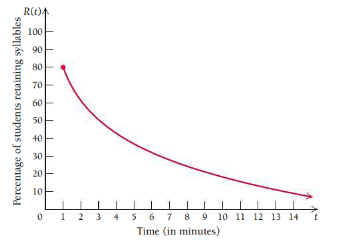
\includegraphics[width=0.5\textwidth]{ /home/mattw/niu/Math211/latexdocs/figures/stuffs.png}
\end{figure}
\bigbreak \noindent
\textbf{Problem 1.} What percentage of students retained the syllables after 1 min.
\bigbreak \noindent
\textit{\textbf{That is,}}
$$ R(1) = 80 - 27\ln{1}$$
\textit{\textbf{since}} $\ln{1} = 0$
\bigbreak \noindent
\textit{\textbf{we have,}}

$$ = 80 - 27(0)$$
$$ = 80 \rightarrow 80\%$$
\bigbreak \noindent
\textbf{Problem 2.} Find $R'(2)$, and explain what it represents.
\bigbreak \noindent
\textit{\textbf{Find}} $f'(x)$
$$ \frac{d}{dx}\left[80 - 27\ln{t}\right]$$
$$ = -\dfrac{27}{x}$$
$$ = -\dfrac{27}{2} = -13.5$$
This result indicates that 2 min after students have been shown the syallables, the percentage of them who retained the syllables is shrinking at the rate of 13.5\$ per minute.
\bigbreak \noindent
\textbf{Problem 3.} When will the percentage of students who retained the syllables drop to 20\%
\bigbreak \noindent
\textit{\textbf{set R(t) = 20 and solve for t}}
$$ 20 = 80 - 27\ln{t}$$
$$ -60 = -27\ln{t}$$
$$\dfrac{20}{9} = \ln{t}$$ 
$$ e^{\frac{20}{9}} = t$$
$$ t \approx 9.23$$
The percentage of students who retained the syllables drops to 20\% after about 9.23 min.
\bigbreak \noindent
\section*{2.4 - Uninhibited and Limited Growth Models}
consider the function given by
$$ f(x) = 2e^{3x}$$
Differentiating, we get
$$ f'(x) = 2e^{3x} \cdot 3$$
$$ = f(x) \cdot 3$$
\bigbreak \noindent
Graphically, this says that the derivative, or slope of the tangent line, is 3 times the function value.
\bigbreak \noindent
Functions of the form 
$$f(x) = ce^{kx}$$
have the property that the derivative is a constant multiple $k$ of the function.
\bigbreak \noindent
\thm{}{
  A function $ y = f(x)$ statisfies
  $$ \frac{dy}{dx} = ky \ \ \ \ or \ \ \ \ f'(x) = k \cdot f(x)$$
  if and only if
  $$ y = ce^{kx} \ \ \ \ or \ \ \ \ f(x) = ce^{kx}$$
}
\q
Find the function that statisfies each equation.
\bigbreak \noindent
\textbf{Problem 1.} $ \dfrac{dA}{dx} = 5A$
\bigbreak \noindent
We know that the desired function must be of the form
$$ A(x) = ce^{kx}$$
Since we have k = 5 in this case, the function is given by $A(x) = ce^{5x}$, where $c$ is an arbitrary constant.

\pagebreak
\noindent\textbf{Problem 2.} $\dfrac{dP}{dt} = kP$
\bigbreak \noindent
The desired function is given by
$$ P(t) = ce^{kt}$$
Where $c$ is an arbitrary constant. As a check, note that
$$ \dfrac{dP}{dt} = ce^{kt} = kP$$
\bigbreak \noindent
\hrule
\bigbreak \noindent
The solutions of the equations in Question 1 are functions. An equation like
$$ \dfrac{dP}{dt} = kP$$
which includes a derivative and which has a function as a solution, is called a \textbf{differential equation}
\bigbreak \noindent
\q
Solve the differential equation
$$ f'(z) = 0.06 \cdot f(z)$$
\sol
$$ f(z) = ce^{0.06z}$$

\bigbreak \noindent
\subsection*{Uninhibited Population Growth}
The differential equation

$$ \dfrac{dP}{dt} = kP \ \ \ \ or \ \ \ \ P'(t) = kP(t), \ \ \ \ \text{with }  k > 0$$
\bigbreak \noindent
Is the model of uninhibited (unrestrained) population growth. In the absence of inhibiting or stimulating factors, a population normally reproduces at a rate proportional to its size, and this is exactly what $\dfrac{dP}{dt} = kP$ says. The only function that satisfies this differential equation is given by
$$ P(t) = ce^{kt}$$
where $t$ is time and $k$ is the rate expressed in decimal notation. Note that
$$ P(0) = ce^{k\cdot0} = ce^{0} = c \cdot 1 = c$$
so c represent the initial population, which we denote as $P_0$
$$ P(t) = P_0e^{kt}$$
\bigbreak \noindent
\hrule
\bigbreak \noindent
\begin{minipage}{0.5\textwidth}
The graph of	
$$ P(t) = P_0e^{kt}, \ \ \ \text{for} \ \ \ k > 0$$
Shows how uninhibited growth produces a ``population explosion'' \\
The constant $k$ is the \textbf{rate of exponential growth}, or the \textbf{exponential growth rate}. This is not the instantaneous rate of change of the population size, which varies according to
$$ \dfrac{dP}{dt} = kP$$
\end{minipage}
\begin{minipage}{0.45\textwidth}
    \incfig[1]{thonk}
    %\caption{thonk}
    %\label{fig:thonk}
\end{minipage}
\pagebreak
\q
Suppose $P_0$, in dollars, is invested in the Von Neumann Hi-Yield Fund, with interest compounded continuously at 7\% per year. That is, at any point in time after $t$ years, the balance $P$, in dollars per year is the growing at the rate
$$ \dfrac{dP}{dt} = 0.07P$$
\bigbreak \noindent
\textbf{Problem 1.} Find the function that satisfies the equation. Write it in terms of $P_0$ and 0.07
\bigbreak \noindent
\textit{\textbf{The function that satisfies the equations is}}

$$ p_0e^{0.07t}$$
\bigbreak\noindent
\textbf{Problem 2.} Suppose that \$10,000 is invested. What is the balance after 1 yr?
\bigbreak \noindent
\textit{\textbf{We have}}

$$P_0 = 10,000 \ \ \ \ and \ \ \ \ t = 1$$
\textit{\textbf{So,}}

$$ P(1) = 10,000e^{0.07(1)}$$
$$ = 10,725.08$$
\bigbreak \noindent
\textbf{Problem 3.} If \$10,000 is invested, how fast is the balance growing at t = 1 yr?
\bigbreak \noindent
\textit{\textbf{For this, we need to find P'(t)}}
$$ \frac{d}{dx}\left[10,000e^{0.07t}\right] = (10,000)\left(0.07e^{0.07t}\right) + \left(e^{0.07t}\right)(0)$$
$$ = 10,000(0.07e^{0.07t})$$
$$ = 700e^{0.07t}$$
\textit{\textbf{Now we solve for P'(1)}}
$$ P'(1) = 700e^{0.07(1)}$$
$$ P'(1) = 750.76$$
\bigbreak \noindent
So, the balance is growing at a rate of \$750.76$ \ \frac{\text{dollars}}{yr}$ at t = 1 yr.
\bigbreak \noindent
\hrule
\bigbreak \noindent
\q
In 1971, Intel Corporation released the Intel 4004 microprocessor, which held 2300 transistors. Since then, the number of transistors on a microprocessor has been growing exponentially at the rate of 0.35, or 35\% per year. That is,
$$ \dfrac{dP}{dt} = 0.35P$$
Where t is the number of years since 1971.
\bigbreak \noindent
\textbf{Problem 1.} Find the function that satisifes this equation. Assume $P_0 = 2300$ and $k = 0.35$
\bigbreak \noindent
\textit{\textbf{The function that satisfies this equation is}}
$$ 2300e^{0.35t}$$
\bigbreak \noindent

\pagebreak
\noindent\textbf{Problem 2.} Estimate the number of transistors on a microprocessor in 2025
\bigbreak \noindent
\textit{\textbf{our value for t is}}
$$ 2025 - 1971$$
$$ t = 54$$
\textit{\textbf{so, we have}}

$$ P_0 = 2300 \ \ \ t = 54 \ \ \ k = 0.35$$
\textit{\textbf{using the equation}}

$$ P_0e^{kt}$$
\textit{\textbf{we have}}

$$P(54) = 2300e^{0.35(54)}$$
$$\approx 371.4 \text{ billion transistors}$$
\bigbreak \noindent
\textbf{Problem 3.} find the rate at which the number of transistors on a microprocessor is changing in 2025.
\bigbreak \noindent
\textit{\textbf{To find the rate of change, we need to find P'(t)}}
$$ \frac{d}{dx}\left[2300e^{.35t}\right] = (2300)(.35e^{.35t}) + (e^{.35t})(0)$$

$$ = 2300(.35e^{.35t})$$
$$ P'(t)= 805e^{.35t}$$
\textit{\textbf{find the rate of change at t = 54}}

$$ P'(54) = 805e^{.35(54)}$$
$$ P'(54) \approx 130 \ \ \text{billion transitors per year}$$
\bigbreak \noindent
\hrule
\bigbreak \noindent
\q
A 1939 comic book with the first appearance of the ``Caped Crusader,'' Batman, sold at auction in Dallas in 2010 for a record \$1.075 million. The comic book originally cost 10\cent (or \$.10). Using the data points (0, \$.10) and (71, \$1,075,000), we can model the increasing value of the comic book. The modeling assumption is that the value V of the comic book grows exponentially, as given by
$$ \dfrac{dV}{dt} = kV$$
\bigbreak \noindent
\textbf{Problem 1.} Find the function that statisfies this equation. Assume $V_0$ = \$.10
\bigbreak \noindent
\textit{\textbf{The function that satisfies the equation is}}
$$ V(t) = 0.10e^{kt}$$
Where V(t) is the comic book's value, in dollars, $t$ years after the start of 1939.
We have made use of the data point (0, \$0.10). Next, we use the data point (71, \$1,075,000) to determine $k$. We solve
$$ V(t) = 0.10e^{kt}, \ \ \ or \ \ \ 1,075,000 = 0.10e^{k(71)}$$
\bigbreak \noindent

\pagebreak
\noindent\textit{\textbf{for k, using natural logarithms}}

$$ 1,075,000 = .10e^{71k}$$
$$ = 10,075,000 = e^{71k}$$
\textit{\textbf{Now we take the natural log of both sides and solve for k}}
$$ \ln{10,075,000} = \ln{e^{71k}}$$
$$ \ln{10,075,000} = 71k$$
$$ \dfrac{\ln{10,075,000}}{71} = k$$
$$ k = 0.228$$
\bigbreak \noindent
\textit{\textbf{So, the desired function is}}
$$ V(t) = 0.10e^{.228t}$$
\bigbreak \noindent
\textbf{Problem 2.} Estimate the value of the comicbook at the start of 2025
\bigbreak \noindent
\textit{\textbf{To find t we do}}

$$ 2025 - 1939$$
$$ t = 86$$
\textit{\textbf{So }}

$$V(86) = 0.10e^{.228(86)}$$
$$ V(86) \approx 32,782,811.85$$
Thus, at the start of 2025, the comic book's value will be about \$32.8 million
\bigbreak \noindent
\textbf{Problem 3.} At what rate, in dollars per year, is the comic books increasing in value at the start of 2025?
\bigbreak \noindent
\textit{\textbf{We need to find V'(t)}}
$$ V'(t) = \frac{d}{dx}\left[0.10e^{.228t} \right]$$
$$ V'(t) = 0.10(.228e^{.228t}) + (e^{.228t})(0)$$
$$ V'(t) = 0.0228e^.228t$$
\textit{\textbf{in 2025, t = 86, so}}
$$ V'(86) = 0.0228e^{.228(86)}$$
$$ V'(86) \approx 7,474,481.102$$
\bigbreak \noindent
Thus, at the start of 2025, the comic book's value is increasing by about \$7.47 million per year

\pagebreak
\subsection*{Models of Limited Growth}
We have seen that the growth model	
$$ P(t) = P_0^{kt}$$
applies to \textit{unlimited}, or \textit{unrestricted}, growth. However, there are often factors that prevent a quantity from exceeding some limiting value L. One model of such \textit{limited}, or \textit{restricted}, growth is
$$ P(t) = \dfrac{l}{1 + Ce^{-Lkt}}, \ \ \ \text{for } k > 0 \ \ \text{and } L > 0$$
Which is called the \textit{logistic equation, or logistic function}
\bigbreak \noindent
\begin{mdframed}
 The differential equation 
 $$ \dfrac{dP}{dt} = kP(L - P)$$
in the model for the logistic function, where L is the upper limit of the population P. The rate of change of the population is directly proportional to the population P and to the remaining room for population growth L - P. The function that solves this differential equation has the simplified form.
$$ P(t) = \dfrac{L}{1 + Ce^{-Lkt}} \ \ \ or \ \ \ P(t) = \dfrac{L}{1 + Ce^{-rt}}$$
where $r = Lk$ and both $k > 0$ and $ L > 0$
\end{mdframed}
\bigbreak \noindent
\pagebreak
\section*{Exponential Decay}
In the equation of population growth,
$$ \dfrac{dP}{dt} = kP$$
The constant k is given by
$$ k = \text{(birth rate)} - \text{(Death rate)}$$
Thus, a population ``grows'' when the birth rate is greater than the death rate and decreases when the birth rate is less than the death rate. For convenience in our computations, we will express a decreasing rate as $-k$, when $k > 0$. The equation
$$ \dfrac{dP}{dt} = -kP, \ \ \text{where } k>0$$
shows P to be \textit{decreasing}, or decaying, as a function of time, and the solution
$$ P(t ) = p_0e^{-kt}$$
shows P to be decreasing exponentially. This is called \textbf{exponential decay.} The amount present initially at t = 0 is again $P_0$
\bigbreak \noindent
\begin{minipage}{0.5\textwidth}
    \incfig[1]{decayy}
\end{minipage}
\begin{minipage}{0.5\textwidth}
    \incfig[1]{raaaawr}
\end{minipage}
\bigbreak \noindent
\subsection*{Radioactive Decay}
Radioactive isotopes decay exponentially; that is, they are continuously decaying at a rate that is proportional to the amount present
\q
Strontium-90 has a continuous decay rate of 2.8\% per year. The rate of change of an amount $N$ of this radioactive isotope is given by
$$ \dfrac{dN}{dt} = -0.028N$$
\bigbreak \noindent
\textbf{Problem 1.} Find the function that satisfies this equation. Let $N_0$ represent the amount present at $ t=0$
\bigbreak \noindent
\textit{\textbf{The function that satisfies this equation is}}
$$ N(t) = N_0e^{-0.028t}$$
\bigbreak \noindent
\textbf{Problem 2.} Suppose that 1000 grams (g) of strontium-90 is present at $ t=90$. How much will remain after 70yr
\bigbreak \noindent
\textit{\textbf{For this we have}}
$$ N(70) = 1000e^{-0.028(70)}$$ 
$$ \approx 140.8584209$$

\pagebreak \noindent
\textbf{Problem 3.} Find the average rate of change of the amount of strontium-90 after 70 yr.
\bigbreak \noindent
\textit{\textbf{We need to find N'(t)}}

$$ N'(t) = \frac{d}{dx}\left[1000e^{-0.028t}\right]$$
$$ N'(t) = 1000(e^{-0.028t} \cdot -0.028) + (e^{-0.028t})(0)$$
$$ N'(t) = 1000(-0.028e^{-0.028t})$$
$$ N'(t) = -28e^{-0.028t}$$
\textit{\textbf{at t = 70, we have}}

$$ -28e^{-0.028(70)}$$
$$ \approx -3.944$$
\bigbreak \noindent
\textbf{Problem 4.} After how long will exactly have of the original 1000 g remain?
\bigbreak \noindent
\textit{\textbf{set half of $P_0$ = to N(t)}}

$$ 500 = 1000e^{-0.028t}$$
\textit{\textbf{solve for t}}

$$ \frac{1}{2} = e^{-0.028t}$$
\textit{\textbf{take the natural log of both sides}}

$$ \ln\frac{1}{2} = \ln{e^{-0.028t}}$$
$$ \ln\frac{1}{2} = -0.028t$$
$$ \frac{\ln\frac{1}{2}}{-0.028t} = t$$
$$ t \approx 25$$
\bigbreak \noindent
\hrule
\bigbreak \noindent
\thm{}{
  The decay rate, $k$, and the half-life, T, are related by
  $$ kT = \ln{2}, \ \ \ or \ \ \ k = \dfrac{\ln{2}}{T} \ \ \ and \ \ \ T = \dfrac{\ln{2}}{k}$$
}
\bigbreak \noindent
\begin{minipage}{0.5\textwidth}
Thus, half-life, T, depends only on decay rate, k, and is independent of the initital population size. The effect of half-life is shown in the radioactive decay curve below. Note that the exponential function gets close to, but never reaches, 0 as $t$ gets larger. Thus, in theory, a radioactive substance never completely decays.
\end{minipage}
\begin{minipage}{0.5\textwidth}
    \incfig[1]{haldlife}
\end{minipage}

\pagebreak
\q
Plutonium-239, a common product of a functioning nuclear reactor, can be deadly to people exposed to it. its decay rate is about $0.0028\%$ per year. What is the half-life?
\bigbreak \noindent
\textit{\textbf{We have}}

$$ k = 0.000028$$
\textit{\textbf{to find t we use}}

$$ T = \dfrac{\ln{2}}{k}$$
\textit{\textbf{So,}}

$$ T = \dfrac{\ln{2}}{0.000028}$$
$$ \approx 24,755$$
\bigbreak \noindent
Thus, the half-life of plutonium-239 is about 24,755 yr
\bigbreak \noindent
\hrule
\bigbreak \noindent
\q
The radioactive element carbon-14 has a half-life of 5730 yr. The percentage of carbon-14 present in the remains of plants and animals is used to determine age. Archaeologists found that the linen wrapping from one of the Dead sea Scrolls had lost 22.3\% of its carbon-14. How old was the linen wrapping?
\bigbreak \noindent
\textit{\textbf{we have t}}
$$ t = 5730$$
\textit{\textbf{we need to find k using the formula,}}
$$ K = \dfrac{\ln{2}}{t}$$
$$ k = \dfrac{\ln{2}}{5730}$$
$$ k \approx 0.00012097$$
\textit{\textbf{Now, we were given that 22.3\% has been lost, however we want what still remains, so}}
$$ 1 - .223 = .777$$
\textit{\textbf{77.7\% still remains. So, }}
$$ .777N_0 = N_0e^{-0.00012097t}$$
$$ .777 = e^{-0.00012097t}$$
\textit{\textbf{Take the natural log of both sides}}
$$ \ln{.777} = \ln{e^{-0.00012097t}}$$
$$ \ln{.777} = -0.00012097t$$ 
$$ t = \dfrac{\ln{.777}}{-0.00012097}$$
$$ t \approx 2086$$
\bigbreak \noindent
Thus, the linen wrapping from the Dead Sea Scroll is about 2086 yr old.

\pagebreak
\q
Following the birth of their granddaughter, Doug and Andrea want to make an initial investment, $P_0$, that will grow to \$10,000 by the child's 20th birthday. Interest is compounded continuously at an annual rate of 4\%
\bigbreak \noindent
\textbf{What should the initial investment be?}
\bigbreak \noindent
\textit{\textbf{We have,}}

$$10,000 = P_0e^{0.4(20)}$$
\textit{\textbf{Solving for $P_0$}}
$$ 10,000 = P_0e^{.8}$$
$$ \dfrac{10,000}{e^{.8}} = P_0$$
$$ P_0 \approx 4493.29$$
Thus, Doug and Andrea should make an inital investment of \$4493.29, which will grow to \$10,000 by the childs 20th birthday.
\begin{figure}[ht]
    \centering
    \incfig[1]{self}
    %\caption{self}
    %\label{fig:self}
\end{figure}
\bigbreak \noindent
Economists call \$4493.29 the \textit{present value} of \$10,000 due 20 yr from now at 4\% per year, compounded continuously. The process of computing present value is called \textbf{discounting}. Another way to pose this problem is to ask ``What should I have invested 20 years ago, at 4\% per year. compounded continuously, in order to have \$10,000 today?''
\bigbreak \noindent
Thus, computing present value can be interpreted as exponential decay from the future back to the present.
\bigbreak \noindent
In general, the present value $P_0$ of an amount P due $t$ years later is found by solving the following equation for $P_0$
$$ p_0e^{kt} = P$$
$$ P_0 = \dfrac{P}{e^{kt}} = Pe^{-kt}$$
\bigbreak \noindent
\thm{}{
  The \textbf{present value} $P_0$ of an amount $P$ due $t$ years later, at interest rate $k$, compounded continuously, is given by
  $$ P_0 = Pe^{-kt}$$
}

\pagebreak
\subsection*{Newton's Law of Cooling}
Consider the following situation. A hot cup of soup, at a temperature of $200^{\circ}$, is placed in a $70^{\circ}$ room. The temperature of the soup decreases over time $t$ according to the model known as Newton's Law of Cooling.
\bigbreak \noindent
\begin{mdframed}
  \begin{large}
   Newton's Law of Cooling 
  \end{large}  
  \bigbreak \noindent
  The temperature $T$ of a cooling object drops at a rate proportional to the difference $ T - C$, where $C$ is the constant temperature of the surrounding medium. Thus,
  $$ \dfrac{dT}{dt} = -k(T - C), \ \ \ for \ \ k > 0 $$
  The function that satisfies equation this is 
  $$ T = T(t) = ae^{-kt} + C$$
\end{mdframed}
\bigbreak \noindent
To check that $T(t) = ae^{-kt} + C$ is the solution, find $\dfrac{dT}{dt}$ and substitute $\dfrac{dT}{dt}$ and $T(t)$ into the equation
$$ \dfrac{dT}{dt} = -k(T - C)$$
\bigbreak \noindent
\q
McDivett's Pie Shoppes, a national chain, finds that the temperature of its freshly brewed coffee is $130^{\circ}$. The company fears that if customers spill hot coffee on themselves, lawsuits might result. Room temperature in the restaurants is generally $72^{\circ}$. The temperature of the coffee cools to $120^{\circ}$ after $4.3 \mathrm{~min}$. McDivett's decides that it is safer to serve coffee at $105^{\circ}$. 
\bigbreak \noindent
\textbf{How long does it take a cup of coffee to cool to $105^{\circ}$ ?}
\bigbreak \noindent
\textit{\textbf{So we have}}

$$ C = 72$$
$$ T(0) = 130$$
\textit{\textbf{So, using the equation}}

$$ T(t) = ae^{-kt} + C$$
\textit{\textbf{We have,}}

$$ 130 = a^{-k(0)} + 72$$
$$ 130 = a + 72$$
$$ a = 58$$
\textit{\textbf{Solve for k, using T(4.3) = 120}}

$$120 = 58e^{-k(4.3)} + 72$$
$$48 = 58e^{-k(4.3)}$$
$$ \dfrac{48}{58} = e^{-k(4.3)}$$
\textit{\textbf{Take the natural log of both sides}}
$$ \ln{\dfrac{48}{58}}  = -4.3k$$
$$ k \approx 0.044$$

\pagebreak \noindent
\textit{\textbf{We now have}}
$$ T(t) = 58e^{-0.044(t)} + 72$$
where $t$ is the cooling time, in minutes. To see how long it will take the coffee to cool to 105, we set T(t) = 105 and solve for t
$$ 105 = 58e^{-0.044t} + 72$$
$$ 33 = 58e^{-0.044t}$$
$$ \dfrac{33}{58} = e^{-0.44t}$$
$$ \ln{\dfrac{33}{58}} = \ln{e^{-0.044t}}$$
$$ \ln{\dfrac{33}{58}} = -0.044t$$
$$ \dfrac{\ln{\dfrac{33}{58}}}{-0.044} = t$$

$$ t \approx 12.8$$
\bigbreak \noindent
So, to reach a temperature of 105, the coffee should cool for about 13 min.
\bigbreak \noindent
\hrule
\section*{Section 2.6 - The Derivatives of $a^x$ and $\log_ax$ }
\bigbreak \noindent
\subsection*{Using Bases Other than 10 or e}
\begin{mdframed}
In many applications involving exponential growth or decay, bases other than 10 or $e$ can be used.
\bigbreak \noindent
For example, in situations where a doubling time or tripling time is known, an exponential function in base 2 or base 3 can be used.
\bigbreak \noindent
Suppose a sample of bacteria in a petri dish doubles in population every 7 hr. That means that in 7 hr an initial population of $P_0$ grows to $2P_0$, and in 14 hr the original population, $P_0$, has  quadrupled and is now $4P_0$, or $2^2 \cdot P_0$. At 21 hr the population after 14 hr has doubled, meaning that the population is now $8P_0$, or $2^3\cdot P_0$. Generalizing, if a population or quantity doubles in T units of time, then after $t$ units of time, the original population has doubled $\dfrac{t}{T}$ times. Using an exponential function with base 2 to model this growth, the population, P(t), after $t$ hours is given by
$$ P(t) = P_0 \cdot 2^{kt}, \ \ \ \ \text{where} \ \ \ k = \dfrac{1}{T}$$
\end{mdframed}
This suggests the following
\subsection*{Base-n Exponential Growth}
If a quantity increases $n$-fold over a fixed period of time $T$, then the quantity $P(t)$ at time $t$ is given by
$$ P(t) = P_0 \cdot {n}^{\frac{t}{T}}$$
Here, increasing a quantity ``2-fold'' is the same as doubling the quantity, increasing a quantity ``3-fold'' is the same as tripling the quantity.
\nt{
  Base-$n$ exponential growth can be expressed in an equivalent form in base $e$, where
  $$ n = e^{\ln{n}}$$
  Both forms have their advantages, as the following two examples illustrate.
}
\q
The number of user accounts for a new photo-sharing app doubles every 3 months. Assume that there were 1000 user accounts when the app became available to the general public (t = 0)
\bigbreak \noindent
\textbf{Problem 1.} Find an exponential function with base 2 that gives the number P(t) of user accounts after t months
\bigbreak \noindent
\textit{\textbf{We have}}

$$ P(t) = 1000 \cdot 2^{\frac{t}{3}}$$
\textit{\textbf{We can write this in terms of base e by using}}

$$ n = e^{\ln{n}}$$
\textit{\textbf{So, we get}}

$$ 1000(e^{\ln{2}})^{\frac{t}{3}}$$
$$ 1000(e^{0.69315})^{\frac{t}{3}}$$
$$ 1000e^{0.23105t}$$
\bigbreak \noindent
\textbf{Problem 3.} What is the number of user accounts after 12 months? Which form of the exponential function is easier to use to find this information?
\bigbreak \noindent
\textit{\textbf{That is}}
$$ P(12) = 1000 \cdot 2^{\frac {13}{3}} = 1000 \cdot 2^4 = 16,000$$
\textit{\textbf{Using base e}}
$$ P(12) = 1000e^{0.23105(12)} = 16,000.2 \approx 16,000$$
The exponential function with base 2 is easier to use, since in 12 months the number of user accounts has doubled 4 times. In this case, a calculator is not necessary to calculate
$$ 1000 \cdot 2 \cdot 2 \cdot 2 \cdot 2 = 16,000$$
\q
Irma invested \$15,000 in a high-yield hedge fund, and after 14 yr, her original investment has tripled. Find exponential functions using base 3 and base $e$ that give the value $A$ of her account after $t$ years. What is the yearly percentage growth rate of her fund? Which exponential function is easier to use to find this information?
\bigbreak \noindent
\textit{\textbf{Using base 3 (n = 3) and tripling time T = 14, we have}}
$$ A(t) = 15,000\cdot 3^{t/14}$$
\textit{\textbf{In base e, this is equivalent to }}
$$ A(t) = 15000(e^{\ln{3}})^{t/14}$$
$$ = 15000(e^{1.0986})^{t/14}$$
$$ = 15000e^{0.0785t}$$
Irma's hedge fund has a yearly percentage growth rate of 7.85\%. Using the function with base $e$, we can read this value directly from the exponent

\pagebreak
\subsection*{The Derivative of $a^x$}
To find the derivative of $a^x$, for $a > 0$, $a \neq 1$, we first express $a^x$ as a power of $e$, using the property

$$ a = e^{\ln{a}}$$
Thus,

$$ a^x = e^{\ln{a^x}}$$
Now, we differentiate both sides:
$$ \frac{d}{dx}a^x = \frac{d}{dx}e^{\ln{a^x}}$$

$$ = \frac{d}{dx}e^{\ln{a^x}}$$
$$ = e^{(\ln{a})x} \cdot \ln a$$
$$ = a^x \cdot \ln a$$
Thus we have the following theorem.
\thm{}{
  $$ \frac{d}{dx}a^x = (\ln a)a^x$$
}
\noindent As a special case, note that

$$ \frac{d}{dx}e^x = e^x \cdot \ln{e} = e^x \cdot 1 = e^x$$
We see that finding derivatives is simpler when using base $e$, since $\ln{e} = 1$
\bigbreak \noindent
\q
Find the derivative of the following functions
\begin{enumerate}
  \item $y = 2^x$ 
  \item $y = (1.4)^x$
  \item $f(x) = 3^{2x+1}$
\end{enumerate}
\bigbreak \noindent \bigbreak \noindent
\textbf{Problem 1.}

$$ \frac{d}{dx}2^x = (\ln{2})2^x$$
\bigbreak \noindent
\textbf{Problem 2.}

$$ \frac{d}{dx}(1.4)^x = (\ln{1.4})(1.4)^x$$
\bigbreak \noindent
\textbf{Problem 3.}
\bigbreak \noindent
\textit{\textbf{Since this function is in the form}}
$$ f(x) = 3^{g(x)}$$
\textit{\textbf{The chain rule applies}}

$$ \frac{d}{dx}3^{2x+1} = (\ln{3})3^{2x+1} \cdot \frac{d}{dx}(2x+1)$$
$$ = \ln 3 \cdot 3^{2x+1} \cdot 2 = 2 \ln{3} \cdot 3^{2x+1}$$

\pagebreak
\subsection*{The Derivative of $log_a{x}$}
Just as the derivative of $a^x$ is expressed in terms of $ln{a}$, so too is the derivative of $log_a{x}$
\bigbreak \noindent
To find this derivative, we first express $log_a{x}$ in terms of $ln{a}$ using the change of base formula
$$ \frac{d}{dx}log_a{x} = \frac{d}{dx} \left(\frac{\log_e{x}}{\log_e{a}}\right)$$
$$ \frac{d}{dx} \left(\frac{\ln{x}}{\ln{a}}\right)$$
$$ = \frac{1}{\ln{a}} \cdot \frac{d}{dx}(\ln{x})$$
$$ = \frac{1}{\ln{a}} \cdot \frac{1}{x}$$
\thm{}{
  $$ \frac{d}{dx}\log_a{x} = \frac{1}{\ln a} \cdot \frac{1}{x} = \frac{1}{x\ln{a}}$$
  
}
As a special case, note that
$$ \frac{d}{dx}(\log_e x) = \frac{1}{\ln e}\cdot \frac{1}{x} = \frac{1}{x}$$
Again, finding derivatives is simpler when using base $e$, since
$$ \frac{1}{\ln e} = \frac{1}{1} = 1$$
\q
Differentiate the following functions
\bigbreak \noindent
\begin{enumerate}
  \item $ y=\log_8{x}$
  \item $ y=\log_x$
  \item $f(x) = \log_3(x^2+1)$
  \item $f(x) = x^3\log_5{x}$
\end{enumerate}
\bigbreak \noindent \bigbreak \noindent
\textbf{Problem 1.}

$$ \frac{d}{dx}\log_8 x$$

$$ = \dfrac{1}{\ln8} \cdot \dfrac{1}{x}$$
$$ = \dfrac{1}{x(\ln{x})}$$
\bigbreak \noindent
\textbf{Problem 2.}

$$ \frac{d}{dx}\log{x}$$

$$ = \frac{1}{\ln{10}} \cdot \dfrac{1}{x}$$
$$ = \dfrac{1}{x(\ln{10})}$$

\pagebreak
\noindent\textbf{Problem 3.}

$$ \frac{d}{dx}\log_3(x^2+1)$$
$$ = \dfrac{1}{\ln{3}} \cdot \dfrac{1}{x^2+1} \cdot 2x$$
$$ = \dfrac{2x}{\ln{3}(x^2+1)}$$
\bigbreak \noindent
\textbf{Problem 4.}

$$ \frac{d}{dx} x^3\log_5{x}$$
$$ = (x^3)(\dfrac{1}{\ln{5}})(\dfrac{1}{x}) + (\log_5{x})(3x^2)$$
$$ = \dfrac{x^3}{x(\ln{5})}+3x^2\log_5{x}$$
$$ = dfrac{x^2}{\ln{5}}+3x^2\log_5{x}$$
\end{document}
